% This is samplepaper.tex, a sample chapter demonstrating the
% LLNCS macro package for Springer Computer Science proceedings;
% Version 2.21 of 2022/01/12
%
\documentclass[runningheads]{llncs}
%
\usepackage[T1]{fontenc}
% T1 fonts will be used to generate the final print and online PDFs,
% so please use T1 fonts in your manuscript whenever possible.
% Other font encondings may result in incorrect characters.
%
\usepackage{graphicx}
% Used for displaying a sample figure. If possible, figure files should
% be included in EPS format.
%
% If you use the hyperref package, please uncomment the following two lines
% to display URLs in blue roman font according to Springer's eBook style:
%\usepackage{color}
%\renewcommand\UrlFont{\color{blue}\rmfamily}
%
 \usepackage[T1]{fontenc}
\usepackage{mathptmx}
\usepackage{titlesec}
{\fontfamily{ptm}\selectfont

% Define formatting for 1st-level heading
\titleformat{\section}
  {\fontsize{12}{14}\bfseries}{\thesection}{1em}{}

% Define formatting for 2nd-level heading
\titleformat{\subsection}
  {\fontsize{10}{12}\bfseries}{\thesubsection}{1em}{}

% Define formatting for 3rd-level heading
\titleformat{\subsubsection}
  {\fontsize{10}{12}\bfseries}{\thesubsubsection}{1em}{}
 
\begin{document}
%
\title{Deep Neural Network Architecture for Cardiac Structures Segmentation}
%
\titlerunning{Deep_Neural_Network_Architecture_For_Cardiac_Structures_Segmentation}
% If the paper title is too long for the running head, you can set
% an abbreviated paper title here
%
\author{Abdul Razzak R Yergatti\inst{1}\and
Vinayak Bhajantri\inst{1}\and
Rahul B Sajjan\inst{1}\and
Satish Chikkamath\inst{1}\and
Kaushik Mallibhat\inst{1}\and 
Nirmala S R.\inst{1}
}

\authorrunning{}
% First names are abbreviated in the running head.
% If there are more than two authors, 'et al.' is used.
%
\institute{\textbf{KLE Technological University Hubballi, India;\\ School of Electronics and Communication Engineering.}\\
\email{abdulrazzakryergattti@gmail.com, vinayakbhajantri2003@gmail.com, sajjanrahul2003@gmail.com, chikkamath@kletech.ac.in, kaushik@kletech.ac.in, nirmala.s@kletech.ac.in}}

\maketitle           % typeset the header of the contribution
%
\begin{abstract}
Determining the cause of cardiovascular illnesses and identifying cardiac-related issues depend heavily on accurate biomedical image segmentation. It primarily aids in the acceleration of illness identification because manual cardiac segmentation by physicians or audiologists can be laborious and unreliable, depending on the experience and competence of the operator. Significant advancements have been made in this field due to the quick growth of deep learning. Nevertheless, traditional automated learning algorithms are unable to divide the whole heart. In turn, the U-Net model for biomedical cardiac medical image segmentation has been applied in this research. The suggested U-Net model uses an encoder that has been enhanced using transfer learning techniques, which enables it to learn from a small quantity of input efficiently. Our primary goal is to classify the myocardium accurately, both left and right valve views in our segmented envision, while segmenting the whole heart image. This component enhances the model’s ability with additional classification and localization, providing improved precision and accuracy in both aspects. Our datasets were acquired from ACDC (Automated Cardiac Diagnosis Challenge). The model performed a dice loss of 0.0185-0.0265 all over the epochs, which is phenomenally good in the segmentation of images.

\keywords{ Whole heart segmentation\and MRI image \and UNet \and Myocardium\and Left ventricle(LV)\and Right ventricle(RV) .}
\end{abstract}
%
%
%
\section{Introduction}
The heart is one of the most important organs in the human body. It is sometimes called the engine of the human body as it is located in the center of the chest and gives blood to every region of the body. Based on data [1], 17.3 million individuals worldwide pass away from cardiovascular ailments each year, with low- and middle-income nations accounting for 80\% of these deaths. Plus, it looks like cardiovascular ailments will take the lives of 23.6 million individuals by 2030 [2]. Modern medical imaging methods including computerized tomographic (CT), MRI, which stands for magnetic resonance imaging, and ultrasound are often used these days to support illness diagnosis

tracking, prognosis, and planning of therapy. The anatomical features and activity of the heart may be quantitatively and qualitatively assessed without invasive operations thanks to these methods.
Nowadays, specialists manually do chamber segmentation[3] using a method called outlining.[3] As of right now, this is the best clinical approach. Manual segmentation[3] takes a lot of time and work, and depending on who does it, might provide different outcomes. Therefore, automation must be incorporated into this system to expedite and streamline the segmentation process [3]. Techniques for distinguishing between the left and right ventricles (LV and RV) using image processing have been developed re- recently, and they can be semi-automatic or fully automated[3]. However, in contrast to LV differentiation, RV separation is anticipated to be substantially more challenging. Since there is currently no solution to the segmentation problem, the RV is usually viewed as less relevant than the +LV [4-5]. One reason for the surge in popularity of deep learning algorithms over the past few decades is their capacity for automated feature recognition.
Nine out of the ten participants that presented a fully automated segmentation approach used CNNs, and eight used a form of Ronneberger et al.’s U-Net. These findings are from the recent MICCAI 2017 ACDC challenge. Cardiologists, radiologists, cardiovascular surgeons, as well as AI developers and data scientists, can benefit from this algorithm. Professionals who create and manage AI tools for cardiac image segmentation further the development of these technologies. Focusing on the precise demarcation of cardiac substructures, including the myocardium, the ventricle to the left, along with the right v, is the paper's main goal. Since these substructures provide vital characteristics including ejection fraction (EF), myocardial mass, and wall thickness, accurate segmentation of these substructures is crucial for therapeutic applications.
With a particular focus on the use of convolutional neural networks (CNNs) and their variations concerning improving the performance metrics such as categorical dice loss and Intersection over Union (IoU) of segmentation tasks, our paper examines and addresses the application of deep learning methods for cardiac image segmentation.
Deep learning is being used to develop new methods for segmenting RV, LV, LA, and RA from cardiac CT and MRI images. These methods are more accurate than traditional methods. Ultrasound images can’t be segmented easily because the availability of these scanned images is less. Magnetic resonance imaging has a major contribution to cardiac image segmentation followed by computed tomography(CT) and ultrasound. Ultrasound image has difficulty in segmenting the image, and adding the datasets has been more of MRI and CT[10].

The structure of the paper appears as listed below- \textbf{\textit{Section2}} talks about the Literature review. \textbf{\textit{Section3 }}describes our proposed methodology. \textbf{\textit{Section4 }}describes the experimentation conducted and its results. \textbf{\textit{Section5}}  concludes this study.



\section{Literature Review}
\label{back}
\subsection{U-net model architecture}
The U-net model architecture has been a go-to architecture for many machine learning tasks since 2015 but more recently it has gained even more popularity down to its incredible performance in image Generation. All of the images in the U-net architecture were initially proposed as a solution to Medical image segmentation problems it was quickly adopted for all sorts of tasks it has a unique structure that makes it particularly effective for tasks with high-resolution inputs and outputs that could be tasks such as image segmentation.

If a U-Net model is trained by passing in images to the model we can produce an
initial guess at the ground truth mask initially guess won’t be accurate we can still use it
to compare against our ground truth label this comparison gives us an error, we can use
to adjust the model’s parameters meaning that the next time we pass in an image we’ll
have a slightly better prediction so why is this model so effective when working with
high-resolution inputs and outputs. The encoder in the U-Net model is in charge of 
retrieving aspects of the input imagery, the decoder is in oversight of sampling intermediate 
features and attracting the final output. 

\subsection{Previous works and details}
\begin{table}[h!]
\centering
\resizebox{\textwidth}{!}{%
\begin{tabular}{|p{2.5cm}|p{2.5cm}|p{2cm}|p{3cm}|p{2.5cm}|p{3.5cm}|p{2cm}|}
\hline
\textbf{Objective of the study} & \textbf{Datasets} & \textbf{Publicly available} & \textbf{ML/DL algorithm} & \textbf{Accuracy / Performance} & \textbf{Challenges} & \textbf{Reference}  \\ \hline
Volume and Ejection Fraction & CT & No & Sparse Regression, CNN & Accuracy - 68 & Accurate detection of Ejection Fraction & [13] \\ \hline
Left Ventricle & MRI & No & CNN, RNN & Accuracy-70, Precision-68 & LV metrics into cardiac function parameters & [14] \\ \hline
LV and cardiac phases & CMRI & No & CNN & Accuracy-74, Precision-65 & Limited availability of datasets for accurate segmentation & [15] \\ \hline
Left Ventricle and Right Ventricle & 2D MRI & No & CNN, U-Net & Accuracy-86 & Segmentation of RV is difficult due to limited datasets & [12] \\ \hline
Segmentation of ventricular boundaries & MRI & No & Dynamic Programming, Gradient Descent & Accuracy-75 & Segmentation of internal cardiac structures & [11] \\ \hline
LV, LA, multi-chamber, Coronary Artery, and Aortic valve segmentation & CT, MRI & Yes & CNN, RNN & Accuracy-95, Precision-86 & Smart Imaging, Deep learning techniques in segmentation & [10] \\ \hline
Shape and Contour segmentation & CT & Yes & DT, CNN & Accuracy-95 & DT not suitable for whole cardiac segmentation & [4] \\ \hline
Segmentation of left ventricle (LV) from echocardiograms & CT, CMR & No & Convolutional LSTM, U-Net & Accuracy-97 & Operator-dependent variability in echocardiography data & [16] \\ \hline
One step detection and image segmentation of whole heart segmentation & CT & Yes & DCNN, U-Net, FCNN, R-CNN & Precision-70 & Processing small patches of volume & [18] \\ \hline
\end{tabular}%
}
\caption{Summary of Studies in Cardiovascular Image Segmentation}
\label{tab:my-table}
\end{table}

\subsection{Related Works}
\label{related}
By paying attention to structure and contour, the author was able to partition the heart on CT images in 2021. the use of deep learning to differentiate the entire cardiovascular system from CT illustrations. Their key area of research included distance transform (DT). Their model centers on the U-Net architecture. created the contour lines- and distance-transform-guided focus network (CDA-Net), an original CNN. Distance transform transition network (DTTN) and the contour changeover network (CTN) was built to construct CDA-Net based on the backbone network. The essential design tenets of CTN and DTTN are coarse shape-prior information and each voxel’s contour probability prediction. There is relatively little penalty energy in the scenario illustrated in (f).To determine the exact boundary line, the contour feature responses aren’t displayed in the background, so the penalty energy (4) acts as an essential part. Hence, contour is of the utmost importance to segmentation.
Techniques based on machine learning have recently been utilized [13], [14], and
[15] to forecast high-level LV/RV details (e.g., volume and ejection \%) without split images. A method for determining the ejection percentage utilizing sparse regression and output correlation has been proposed by Gu et al. [13]. A network called Indices-Net has been developed by Xue et al. [14] and can instantly determine the myocardium area, the LV size, and the six regional wall thicknesses. A CNN has been included in Indices-Net for regression and a deep convolution autoencoder for image representation. By employing two recurrent neural networks to explain the temporal dynamics of cardiopulmonary sequences and a CNN for picture representation,
Xue et al. [15] substantially enhanced the model that could forecast LV indices and the cardiac phase in parallel. It ought to be pointed out that while it could be done to quantify the LV/RV parameters without localizing the contours due to cardiac diagnos- tics revolving around widely recognized physiological parameters, physicists normally need contour maps to figure out when the values for cardiac quantification spring from truly physiological measurements.
To separate the right ventricle, they limited the form before deploying a U-net network in this research [3]. The RV form's prior probability is set by the size of the RV endocardium county. Network coefficients for loss then include the prior probability by measuring the KL divergence between the prediction probability and the prior probability. A shorter and better-performing network can potentially be trained by integrating the segmentation network with registration.
A potent and trustworthy deformable model has been published by A Gupta, and it incorporates approaches to dividing up ventricular boundaries using cardiac MR images. Dynamic programming, based on an algorithm by A. Gupta, was integrated into multiscale analysis [11]. Beyond that, it is sensitive to having particularly acute ori- gins strategies. In just ten minutes, the algorithm has been embedded in a user interface that kinds, packs, interprets, and portrays cardiac details. With close to 1,000 photos, a Gupta examined the deformable model, and the results were good [11]. Intending to gather the outcomes of checking out a patient study, A Gupta created a protocol with 12 phases and 10 slices for each phase [11]. The above approach is used to minimize the energy of the final form. The algorithm hinges on gradient descent conduct and dynamic programming. The two algorithms are provided in this model. Energy min- imization is the objective of these algorithms. The first conduct covered the steepest descent with only local optimization. Dynamic programming is essential for the second algorithm. A non-iterative position is utilized in the second. An approach using adaptive programming has been developed to stop the local minima concern. The larger search space, which relies on dynamic programming, is also utilized for spatial dissemination.The strategy ensures that the specific user search area obtains suitable contours. The patient’s cardiac mass, as described by a Gupta, was 216.53 grams.
The paper [10] points out the advantages and persistent problems with current deep learning-based segmentation methods that prevent their general clinical use. Additionally, it provides a summary of the most recent advancements in deep learning methods for segmenting cardiac images in the three modalities that are most commonly employed in clinical applications. The primary subjects of the author's discussion included the multichamber, LV, LA, and segmentation of the aortic valve. Pre- and post-processing are part of the CNN approach, which is utilized to segment the coronary arteries. This paper illustrates the challenges and prospective directions for deep learning techniques research. This study demonstrates the difficulties and potential research areas for deep learning methods. They gave a quick overview of upcoming projects like Smart Imaging, Data Harmonization, and Data Privacy to develop deep learning algorithms. This study [10] is the result of referencing one hundred publications, all of which are different segmentation projects carried out by academics.

\section{Proposed Methodology}
\label{proposed}
\begin{figure*}[h]
    \centering
    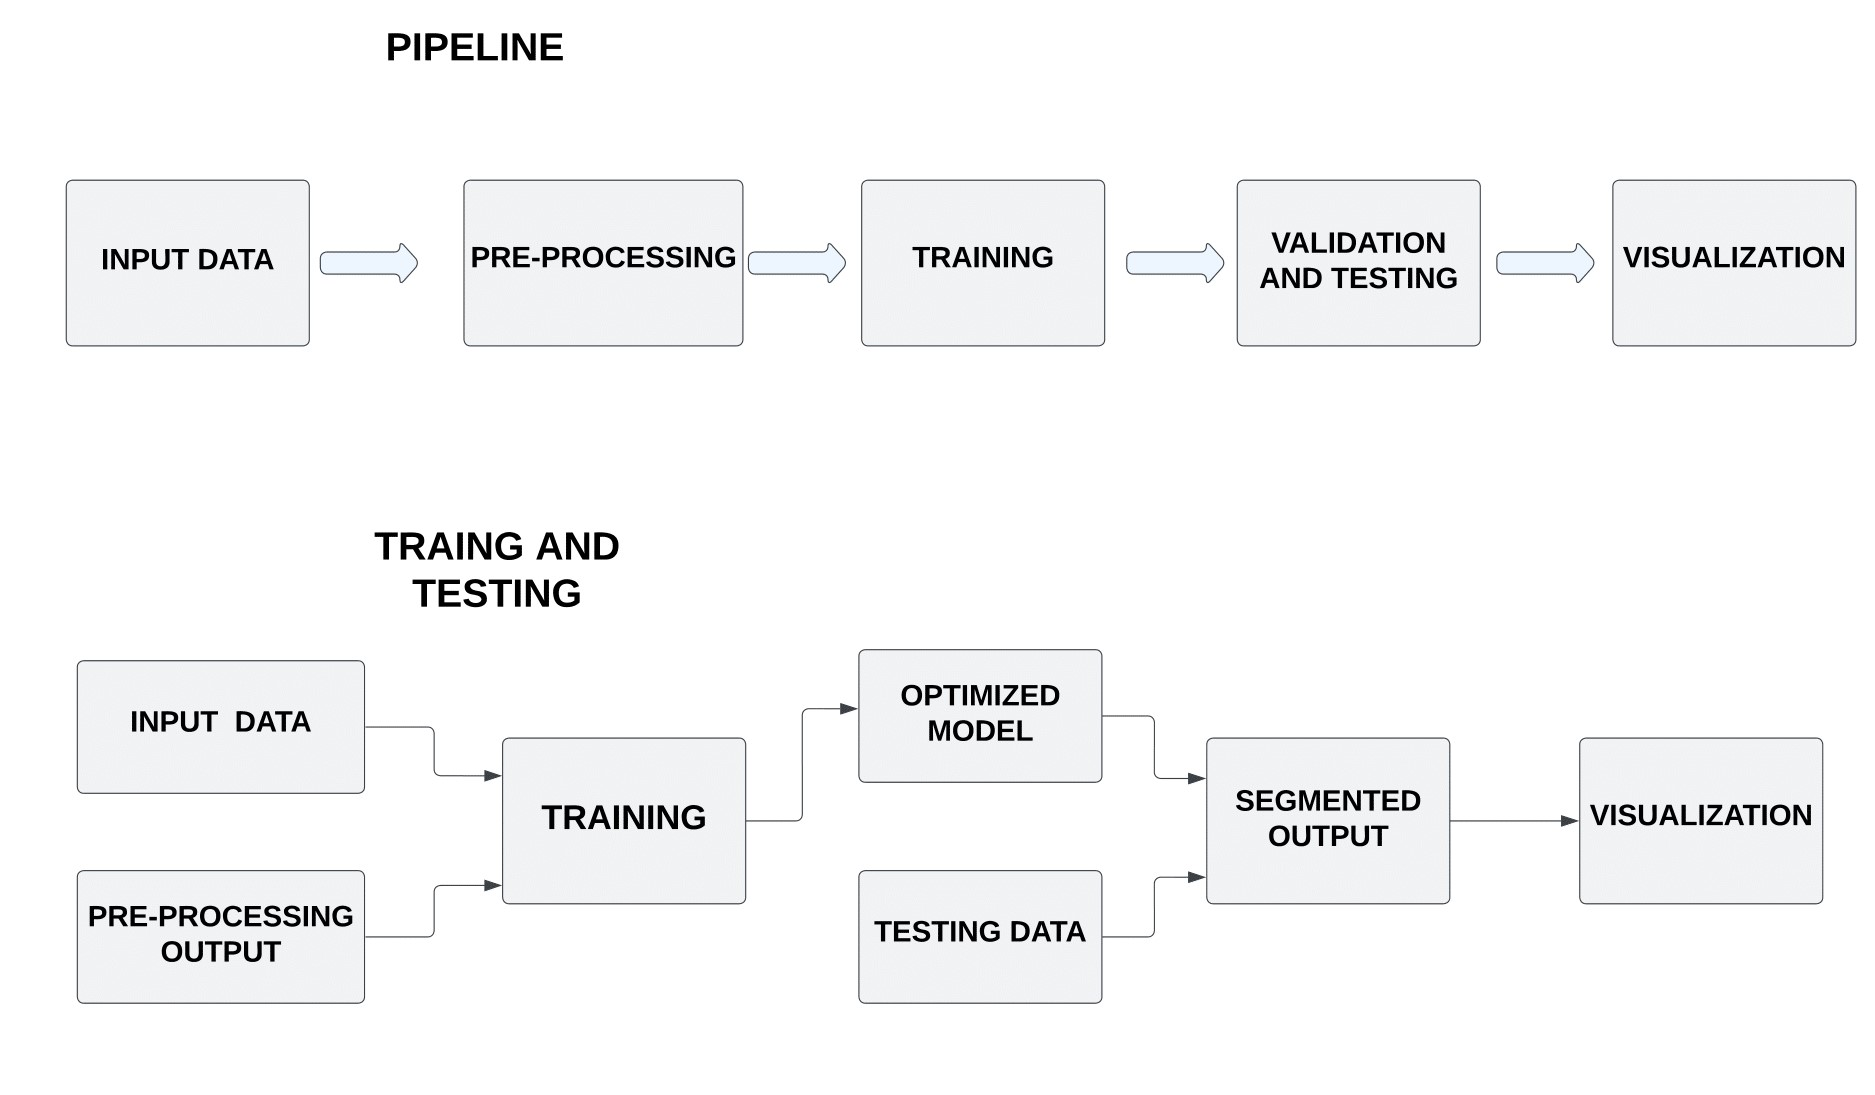
\includegraphics[width=\textwidth]{pipeline.jpg}
    \caption{Flow diagram of the proposed model}
    \label{fig: flow}
\end{figure*}
In the context of deep Neural Network Architecture for Cardiac Structures Segmentation, more advanced technology has been used nowadays but there are certain drawbacks :
\begin{itemize}
    \item Variations in anatomical (cardiac) structures among individuals can make segmentation challenging.
    \item Complexities in heart size, shape, and delineating various cardiac structures such as chambers, valves, and vessels.
    \item   Noise, artifacts, variations in imaging modalities (like MRI and CT scans), and motion-related issues in cardiac imaging affect segmentation accuracy.

\end{itemize}
To counter a few drawbacks, the following are our contributions to this project : 
\begin{itemize}
    \item Dataset: The Automated The amount of blood flowing Diagnosis Challenge (ACDC) provided the dataset. Comparing the precision of automated approaches for the segmentation of the anterior left LV endocardium and epicardium as the right ventricular endocardium is the end-diastolic ACDC challenge. for occurrences of the end-diastolic and end-systolic phases. ventricular Real clinical exams from the University Hospital of Dijon (France) have been utilized to build the whole ACDC dataset. Data were appropriately anonymized and handled according to the guidelines provided by the Hospital about Dijon's local ethics committees. To: (1) effectively train artificial intelligence algorithms; and (2) properly examine disparities that occur in the primary physiological parameters (the latter volume and eject percent), our dataset contains enough samples of many well-defined illnesses. taken from the film MRI. The dataset, which includes 150 exams from different patients, is divided into 5 equally distributed subgroups (four diseased and one healthy subject group). The public is permitted to obtain the dataset.
    \item U-Net: –We have used the U-Net model architecture to train our model. Mainly used for medical image segmentation that can more accurately segment images using a smaller amount of training data. Can be used for image localization, which helps in predicting the image pixel by pixel. It also achieves good performance on very different biomedical segmentation making it flexible and adaptable to our cardiac image segmentation task.
\end{itemize}

\subsection{Feature Extraction}
To extract the features of the input dataset, we looked at the common libraries. Both Albumentations and Scikit-Image were the available options. A Python module called Albumentations is used to compose the dataset file. It provides a variety of features to transform into a composed image file. Functions from Albumentations are used for rotation, flipping with scale limit, shift limit, border mode and rotate limit. Each input image is composed and transformed and given to training, validation, and testing. The hyperparameters which are used in optimization are used to transform the image files.
   
\subsection{Classifier Training}
As part of the preprocessing, the characteristics were extracted from the Automated Cardiac Diagnosis Challenge (ACDC) dataset, and divided into training, validation, and testing sets. The U-Net model was optimized using the Adam optimizer after 100 training iterations with a learning rate of 0.008 and a loss function of categorical dice-loss. Observing the model’s performance while it was being trained, we adjusted the hyperparameters to increase the model’s precision. The model was trained and then quantized to make it a lightweight model that could be used on validation and testing sets. The effectiveness of our approach cannot be achieved with traditional algorithms thus the algorithms such as Albumentations, Dataloder, EfficientNet-B4 Encoder, and performance metrics such as Categorial Dice-loss, Cross-Entropy loss, and (IOU) Intersection Over Union.


\subsection{Comparison with other models}
As we are segmenting the whole heart image the U-Net architecture which was specially developed for the bio-medical image segmentation will be less time-consuming and more perspicuous images will be segmented at the output. The traditional machine learning algorithms for example Logistic Regression, Random forest, (SVM) Support vector machines, and Decision-Tree-Classifier will not be more accurate. Many people have used the FCN model but the drawback is the model can only predict the specific part of the heart. As we want to segment the whole heart into a single segmented image the U-Net model will be more helpful for training the encoder which consists of transfer learning methods, allowing it to effectively learn from a limited amount of data.

\section{Experimentation and Results}
\label{exp}
The training of Anatomy-Guided Cardiac Image Segmentation is done on Google Colab which has NVIDIA K80 / T4 @1.59GHz GPU with 16GB RAM.

\subsection{Dataset}
 One of the major problems in cardiac image segmentation was the availability of the dataset. Thus we have collected a total of 2000 masked images and 2000 heart images. The dataset consists of five classes (normal case, dilated cardiomyopathy, abnormal right ventricle, heart failure with infarction, and hypertrophic cardiomyopathy). The dataset, sourced from clinical exams at the University Hospital of Dijon, consisting of 150 examinations from various patients, is divided into five equally sized subgroups (4 pathological and 1 healthy). Fig. 2 represents the segmented image of the heart. Taking the same into picture we have used 1000 images for training our model, 800 images for testing, and 200 images for validation.

 \begin{figure}[h]
    \centering
    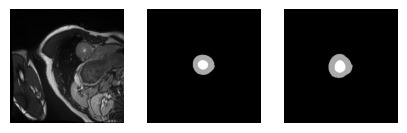
\includegraphics[scale=0.6]{validationset1.jpg}
    \centering
    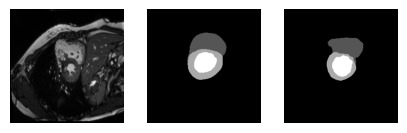
\includegraphics[scale=0.6]{validationset2.jpg}
    \caption{Input Image, Ground truth Image, and segmented Image}
    \label{fig:spectogram}
\end{figure}
After the Executing validation snippet, we got the Ground truth image and segmented image as shown in Fig. 2, the validation set used for our model’s architecture has 3 images namely the input image or original image which we have used for image recognition or object detection. Ground truth image is used as a reference for the ideal output that the model aims to achieve during training or evaluation. The ground truth provides the correct annotations or labels for each pixel or region in an image. The segmented or output image is the output generated by model architecture. In image segmentation, the goal is to partition an input image into meaningful regions or segments. Each segment corresponds to a specific region of interest. During validation, the input images from the validation set are processed by the trained model, and the model’s predictions (segmented images) are compared against the ground truth images to evaluate its performance metrics.
 
 \begin{figure}[h]
    \centering
    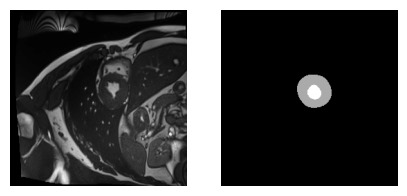
\includegraphics[scale=0.4]{testingset1.jpg}
    \centering
    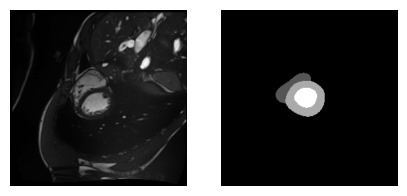
\includegraphics[scale=0.4]{testingset2.jpg}
    \caption{Input heart Image and segmented heart Image}
    \label{fig:spectogram}
\end{figure}
Fig. 3 Shows the testing set which has the input heart image and the segmented heart image as the output image. The input images are raw data that we have used during the testing of our model and the output is then compared with the ground truth image during the validation phase to assess the performance of the model.
\medskip

\begin{figure}[h]
    \centering
    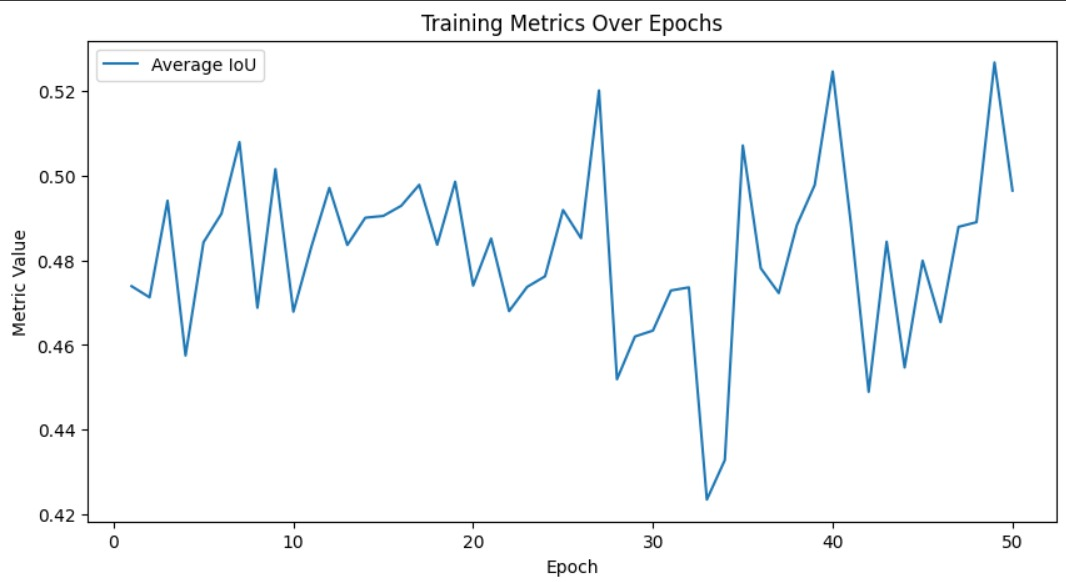
\includegraphics[scale=0.2]{iou.jpeg}
    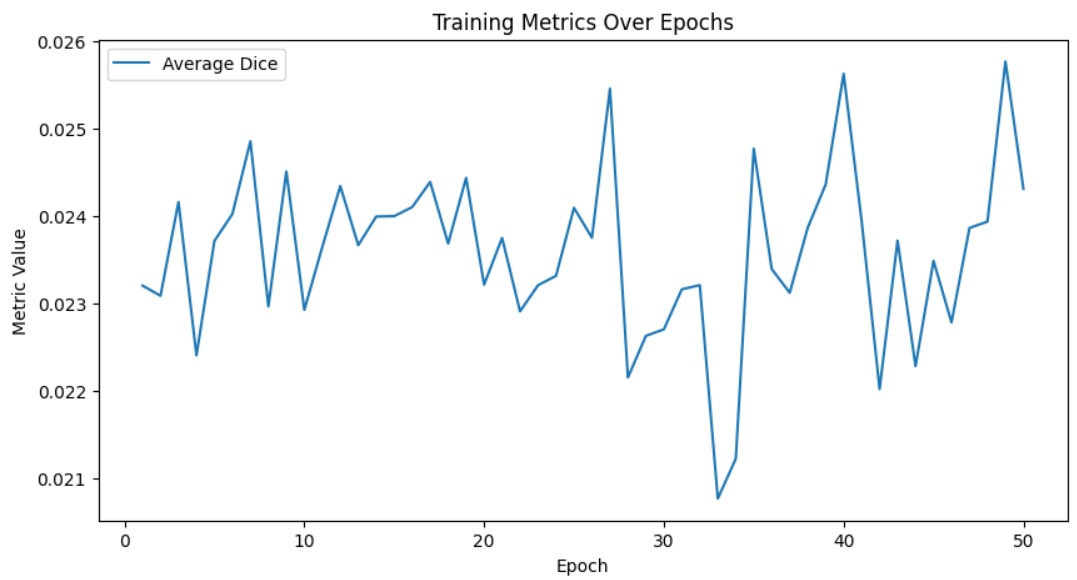
\includegraphics[scale=0.2]{dice_train.jpg}
    \caption{IOU Score Epoch.}
    \label{fig:res}
    \caption{Dice Loss Over Epochs.}
    \label{fig:res}
\end{figure}
We Used performance metrics named IOU Score and Dice Loss Over Epochs. Since our model’s accuracy, can’t be measured therefore performance matrices are used to calculate the correctness of the segmented image. The accuracy value is difficult to get for the segmentation of the images, so to verify we can use these performance metrics which enable us to the correct direction.

\section{Conclusion}
\label{con}
The project objective looks to segment the cardiac image using deep learning techniques. Our method entails several phases, from cardiac images to getting the appropriate segmented image. In conclusion, it has been demonstrated that utilizing CNN to segment the cardiac images with their ground truth mask is a successful method. According to the model’s findings, the model performed a dice loss of 0.0185-0.0265 all over the epochs, which is phenomenally good in the segmentation of images. The model’s deployment in the medical field shows how this could work in real-world phenomena. With a limited dataset, we segmented the cardiac image into three parts. However, it could be advantageous to go into deeper segmentation for the end users if a model fills the current gap.


\cite{re1,re2,re3,re4,re5,re6,re7,re8,re9,re10,re11,re12,re13,re14,re15,re16,re18,re17,re19}
\bibliography{refer}
\bibliographystyle{unsrt}
\end{document}
